\documentclass[10pt]{article}

\usepackage{amsthm}
\usepackage{amsmath}
\usepackage{amssymb}
\usepackage{mathtools}
\usepackage{graphicx}
\usepackage[colorinlistoftodos]{todonotes}
\usepackage{url}
\usepackage{xcolor}

\usepackage{pgfplots}

\usepackage[left = 1cm, top = 1cm, bottom = 2cm, right = 1cm, nohead, nofoot]{geometry}

\pgfplotsset{width=20cm, compat=1.9}

\newcommand{\C}{\mathbb{C}}  % Complex
\newcommand{\R}{\mathbb{R}}  % Real
\newcommand{\Z}{\mathbb{Z}}  % Integers
\newcommand{\N}{\mathbb{N}}  % Naturals

\newcommand{\A}{\mathbb{A}}
\newcommand{\K}{\mathbb{K}}

\title{$\A$dvanced $\C$alculus}
\author{$\C$ason $\K$onzer}
\date{October 30, 2021}



\begin{document}
\maketitle

\newpage

%%%%%%%%%%%%%%%%%%%%%%%%%%%%%%%%%%%%%%%%%%%%%%%%%%%%%%%%%%%%%%%%%%%%%%%%%%%%%%%%%%%%%%%%%%%%%%%%
%%%%%%%%%%%%%%%%%%%%%%%%%%%%%%%%%%        Problem #1       %%%%%%%%%%%%%%%%%%%%%%%%%%%%%%%%%%%%%
\section{\underline{}}
\label{sec: Problem 1}
\noindent
Derive a formula for $ \mathcal{F}_c\{f^{(4)}(x)\} $ in terms of $ \mathcal{F}_c\{f(x)\} $ and $ \mathcal{F}_s\{f(x)\} $. \\
\vspace{2.5mm}
\hrule 

\vspace{7.5mm}

\noindent
\textbf{Solve} iteratively. \\

\begin{itemize}
    \item $ \mathcal{F}_c\{f^{(4)}(x)\} = \mathcal{F}_c\{(f^{(3)}(x))^\prime\} 
    = \mathcal{F}_c\{(f^{\prime\prime}(x))^{\prime\prime}\} 
    = \mathcal{F}_c\{(f^{\prime}(x))^{(3)}\} $.
    \vspace{2.5mm}
    \item $ \displaystyle \mathcal{F}_c\{f^{\prime}(x)\} = w\mathcal{F}_s\{f(x)\} - \sqrt{\dfrac{2}{\pi}}f(0) \ \ 
    ; \ \ \mathcal{F}_s\{f^{\prime}(x)\} = -w\mathcal{F}_c\{f(x)\} $.
    \vspace{2.5mm}
    \item $ \displaystyle \mathcal{F}_c\{f^{\prime\prime}(x)\} 
    = \mathcal{F}_c\{(f^{\prime}(x))^{\prime}\} 
    = w\mathcal{F}_s\{f^{\prime}(x)\} - \sqrt{\dfrac{2}{\pi}}f^{\prime}(0) $.
    \vspace{2.5mm}
    \subitem $ \displaystyle = -w^2\mathcal{F}_c\{f(x)\} - \sqrt{\dfrac{2}{\pi}}f^{\prime}(0) $.
    \vspace{2.5mm}
    \item $ \displaystyle \mathcal{F}_c\{f^{(3)}(x)\} 
    = \mathcal{F}_c\{(f^{\prime\prime}(x))^{\prime}\} 
    = -w^2\mathcal{F}_c\{f^{\prime}(x)\} - \sqrt{\dfrac{2}{\pi}}f^{\prime\prime}(0) $.
    \vspace{2.5mm}
    \subitem $ \displaystyle = -w^3\mathcal{F}_s\{f(x)\} + w^2\sqrt{\dfrac{2}{\pi}}f(0) - \sqrt{\dfrac{2}{\pi}}f^{\prime\prime}(0) $.
    \vspace{2.5mm}
    \item $ \displaystyle \mathcal{F}_c\{f^{(4)}(x)\} 
    = \mathcal{F}_c\{(f^{(3)}(x))^{\prime}\} 
    = -w^3\mathcal{F}_s\{f^{\prime}(x)\} + w^2\sqrt{\dfrac{2}{\pi}}f^{\prime}(0) - \sqrt{\dfrac{2}{\pi}}f^{\prime\prime\prime}(0) $.
    \vspace{2.5mm}
    \subitem $ \displaystyle = w^4\mathcal{F}_c\{f(x)\} + w^2\sqrt{\dfrac{2}{\pi}}f^{\prime}(0) - \sqrt{\dfrac{2}{\pi}}f^{\prime\prime\prime}(0) $.
\end{itemize}

\newpage

%%%%%%%%%%%%%%%%%%%%%%%%%%%%%%%%%%%%%%%%%%%%%%%%%%%%%%%%%%%%%%%%%%%%%%%%%%%%%%%%%%%%%%%%%%%%%%%%
%%%%%%%%%%%%%%%%%%%%%%%%%%%%%%%%%%        Problem #2       %%%%%%%%%%%%%%%%%%%%%%%%%%%%%%%%%%%%%
\section{\underline{}}
\label{sec: Problem 2}
\noindent
Find $ \mathcal{F}_s\{f(x)\} $ for an odd function with $ f(x)=\left\{\begin{array}{ll}
    x & \mbox{if} \quad -1 < x < 1\\
    -1 & \mbox{if} \quad -2 < x < -1\\
    1 & \mbox{if} \quad 1 < x < 2\\
    0 & \mbox{if} \quad x < -2, \ x > 2 \\
\end{array}
\right. $.  \\
\vspace{2.5mm}
\hrule 

\vspace{7.5mm}

\begin{center}
    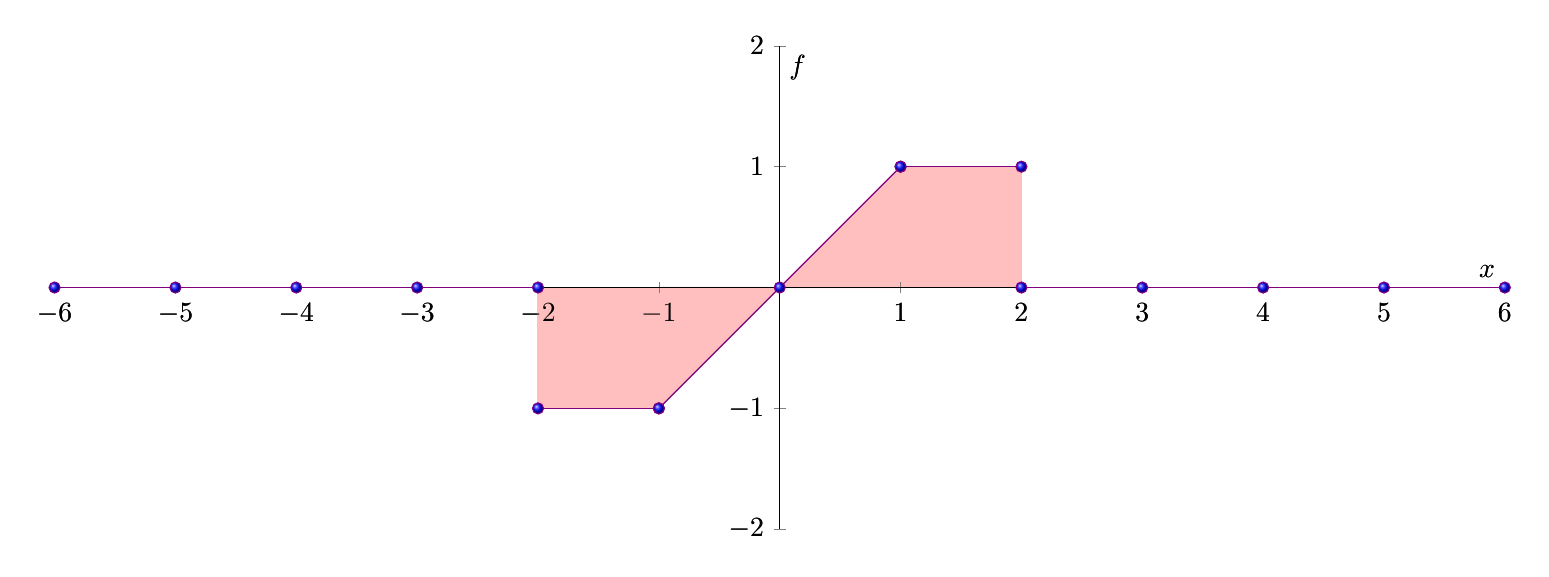
\begin{tikzpicture}
        \begin{axis}[
            xlabel = $ x $, ylabel = $ f $,
            xmin = -6, xmax = 6,
            ymin = -2, ymax = 2,
            try min ticks =  1,
            axis equal image = true,
            axis x line=center,
            axis y line=center,
            axis line style = -,
            ]
            \addplot[
                no marks,
                color = pink,
                fill
                ]
                expression[
                    domain = -1 : 1,
                    samples = 5
                    ]
                    {x}
                \closedcycle
            ;
            \addplot[
                no marks,
                color = pink,
                fill
                ]
                expression[
                    domain = -2 : -1,
                    samples = 5
                    ]
                    {-1}
                \closedcycle
            ;
            \addplot[
                no marks,
                color = pink,
                fill
                ]
                expression[
                    domain = 1 : 2,
                    samples = 5
                    ]
                    {1}
                \closedcycle
            ;
        \end{axis}
        \begin{axis}[
            xlabel = $ x $, ylabel = $ f $,
            xmin = -6, xmax = 6,
            ymin = -2, ymax = 2,
            try min ticks =  1,
            axis equal image = true,
            axis x line=center,
            axis y line=center,
            axis line style = -,
            ]
            \addplot[
                mark = ball,
                color = violet
                ]
                expression[
                    domain = -1 : 1,
                    samples = 3
                    ]
                    {x}
            ;
            \addplot[
                mark = ball,
                color = violet
                ]
                expression[
                    domain = 1 : 2,
                    samples = 2
                    ]
                    {1}
            ;
            \addplot[
                mark = ball,
                color = violet
                ]
                expression[
                    domain = -2 : -1,
                    samples = 2
                    ]
                    {-1}
            ;
            \addplot[
                mark = ball,
                color = violet
                ]
                expression[
                    domain = 2 : 6,
                    samples = 5
                    ]
                    {0}
            ;
            \addplot[
                mark = ball,
                color = violet
                ]
                expression[
                    domain = -6 : -2,
                    samples = 5
                    ]
                    {0}
            ;
        \end{axis}
    \end{tikzpicture} \\
\end{center}

\noindent
\textbf{Solve}  \\

\begin{itemize}
    \item $ \displaystyle \mathcal{F}_s\{f(x)\} = \sqrt{\dfrac{2}{\pi}} \int_{0}^{\infty} f(x) \sin(vx) \,dx $
    \subitem  $ \displaystyle = \sqrt{\dfrac{2}{\pi}} \int_{0}^{1} x \sin(vx) \,dx + \sqrt{\dfrac{2}{\pi}} \int_{1}^{2} 1 \sin(vx) \,dx + \sqrt{\dfrac{2}{\pi}} \int_{2}^{\infty} 0 \sin(vx) \,dx $
    \subitem  $ \displaystyle = \sqrt{\dfrac{2}{\pi}}x \int_{0}^{1} \sin(vx) \,dx + \sqrt{\dfrac{2}{\pi}} \int_{1}^{2} \sin(vx) \,dx 
    = \sqrt{\dfrac{2}{\pi}} \Big[\dfrac{\sin{wx}}{w^2} - \dfrac{x\cos{wx}}{w} \Big|_{0}^{1} \Big] \,dx - \sqrt{\dfrac{2}{\pi}} \Big[\dfrac{\cos{wx}}{w} \Big|_{1}^{2} \Big] $
    \subitem  $ \displaystyle = \sqrt{\dfrac{2}{\pi}}x \Big[\dfrac{\sin{w}}{w^2} - \dfrac{\cos{w}}{w} - \dfrac{\cos{2w}}{w} + \dfrac{\cos{w}}{w} \Big] $
    \subitem  $ \displaystyle = \sqrt{\dfrac{2}{\pi}}x \Big[\dfrac{\sin{w}}{w^2} - \dfrac{\cos{2w}}{w} \Big] $
\end{itemize}

\newpage

%%%%%%%%%%%%%%%%%%%%%%%%%%%%%%%%%%%%%%%%%%%%%%%%%%%%%%%%%%%%%%%%%%%%%%%%%%%%%%%%%%%%%%%%%%%%%%%%
%%%%%%%%%%%%%%%%%%%%%%%%%%%%%%%%%%        Problem #3       %%%%%%%%%%%%%%%%%%%%%%%%%%%%%%%%%%%%%
\section{\underline{}}
\label{sec: Problem 3}
\noindent
Find $ \mathcal{F}\{f(x)\} $, where $ f(x)=e^{-|x|} $ for $ -\infty < x < \infty $. (Hint: you cannot use a table for this). \\
\vspace{2.5mm}
\hrule 

\vspace{7.5mm}

\begin{center}
    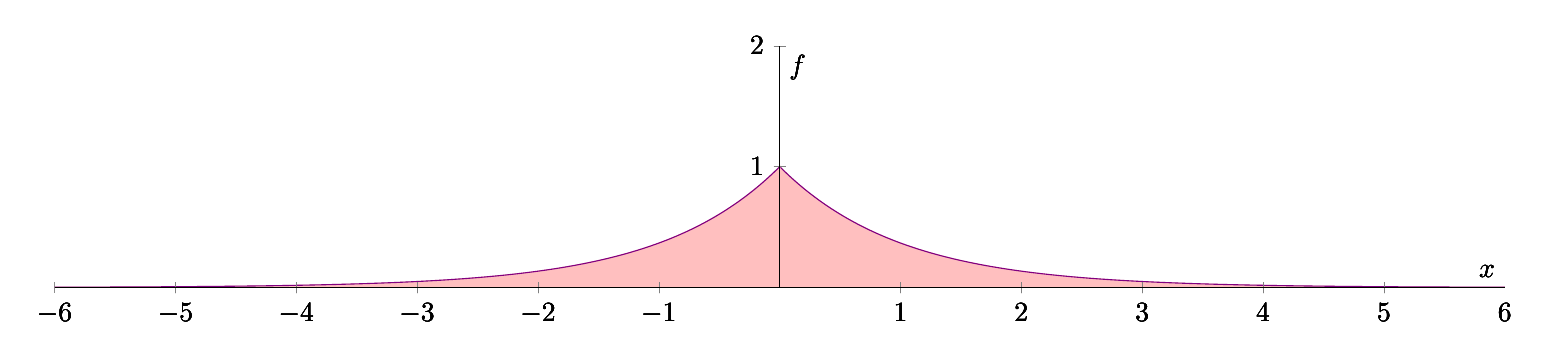
\begin{tikzpicture}
        \begin{axis}[
            xlabel = $ x $, ylabel = $ f $,
            xmin = -6, xmax = 6,
            ymin = 0, ymax = 2,
            try min ticks =  2,
            axis equal image = true,
            axis x line=center,
            axis y line=center,
            axis line style = -
        ]
            \addplot[
                no marks,
                color = pink,
                fill
            ]
                expression[
                domain = 0 : 6,
                samples = 500
                    ]
                    {pow(e,-x)}
                \closedcycle
            ;
        \end{axis}
        \begin{axis}[
            xlabel = $ x $, ylabel = $ f $,
            xmin = -6, xmax = 6,
            ymin = 0, ymax = 2,
            try min ticks =  2,
            axis equal image = true,
            axis x line=center,
            axis y line=center,
            axis line style = -
        ]
            \addplot[
                no marks,
                color = violet
            ]
                expression[
                domain = 0 : 6,
                samples = 500
                    ]
                    {pow(e,-x)}
            ;
        \end{axis}
        \begin{axis}[
            xlabel = $ x $, ylabel = $ f $,
            xmin = -6, xmax = 6,
            ymin = 0, ymax = 2,
            try min ticks =  2,
            axis equal image = true,
            axis x line=center,
            axis y line=center,
            axis line style = -
        ]
            \addplot[
                no marks,
                color = pink,
                fill
            ]
                expression[
                domain = -6 : 0,
                samples = 500
                    ]
                    {pow(e,x)}
                \closedcycle
            ;
        \end{axis}
        \begin{axis}[
            xlabel = $ x $, ylabel = $ f $,
            xmin = -6, xmax = 6,
            ymin = 0, ymax = 2,
            try min ticks =  2,
            axis equal image = true,
            axis x line=center,
            axis y line=center,
            axis line style = -
        ]
            \addplot[
                no marks,
                color = violet
            ]
                expression[
                domain = -6 : 0,
                samples = 500
                    ]
                    {pow(e,x)}
            ;
        \end{axis}
        \begin{axis}[
            xlabel = $ x $, ylabel = $ f $,
            xmin = -6, xmax = 6,
            ymin = 0, ymax = 2,
            try min ticks =  2,
            axis equal image = true,
            axis x line=center,
            axis y line=center,
            axis line style = -
        ]
            ;
        \end{axis}
    \end{tikzpicture} \\
\end{center}

\vspace{2.5mm}
\noindent
\textbf{Solve} \\

\begin{itemize}
    \item $ \displaystyle \mathcal{F}\{f(x)\} = \sqrt{\dfrac{1}{2\pi}} \int_{-\infty}^{\infty} f(x) e^{-iwx} \,dx = \sqrt{\dfrac{1}{2\pi}} \int_{-\infty}^{\infty} e^{-|x|}e^{-iwx} \,dx  $
    \vspace{2.5mm}
    \subitem $ \displaystyle = \sqrt{\dfrac{1}{2\pi}} \int_{-\infty}^{0} e^{x - iwx} \,dx + \sqrt{\dfrac{1}{2\pi}} \int_{0}^{\infty} e^{-x - iwx} \,dx 
    = \sqrt{\dfrac{1}{2\pi}} \int_{-\infty}^{0} e^{x(1 - iw)} \,dx + \sqrt{\dfrac{1}{2\pi}} \int_{0}^{\infty} e^{-x(1 + iw)} \,dx $
    \vspace{2.5mm}
    \subitem $ \displaystyle = \sqrt{\dfrac{1}{2\pi}} \Big[\dfrac{e^{x(1 - iw)}}{1 - iw} \Big|_{-\infty}^{0}\Big] + \sqrt{\dfrac{1}{2\pi}} \Big[\dfrac{e^{-x(1 + iw)}}{-1 - iw} \Big|_{0}^{\infty}\Big] 
    = \sqrt{\dfrac{1}{2\pi}} \Big[\dfrac{e^{0(1 - iw)}}{1 - iw} - \dfrac{e^{-\infty(1 - iw)}}{1 - iw} + \dfrac{e^{-\infty(1 + iw)}}{-1 - iw} - \dfrac{e^{0(1 + iw)}}{-1 - iw}\Big] $
    \vspace{2.5mm}
    \subitem $ = \sqrt{\dfrac{1}{2\pi}} \Big[\dfrac{1}{1 - iw} - \dfrac{0}{1 - iw} + \dfrac{0}{-1 - iw} - \dfrac{1}{-1 - iw}\Big] 
    = \sqrt{\dfrac{1}{2\pi}}\Big[\dfrac{(-1 - iw) - (1 - iw)}{(1 - iw)(-1 - iw)}\Big] 
    = \sqrt{\dfrac{1}{2\pi}}\Big[\dfrac{-2}{-1 - w^2}\Big] $
    \vspace{2.5mm}
    \subitem $ \displaystyle = \dfrac{2}{\sqrt{2\pi}(1 + w^2)} $.
\end{itemize}

\end{document}



%%%%%%%%%%%%%%%%%%%%%%%%%%%%%%%%%%%%%%%%%%%%%%%%%%%%%%%%%%%%%%%%%%%%%%%%%%%%%%%%%%%%%%%%%%%%%%%%
%%%%%%%%%%%%%  Comments - October 30, 2021 Advanced Calculus Written Home Work #5  %%%%%%%%%%%%%